\documentclass[12pt,a4paper]{article}

\usepackage{amsfonts, amsthm, amsmath, amssymb}

\usepackage{booktabs}
\renewcommand{\arraystretch}{1.3}

\usepackage{float}

\usepackage{hyperref}
\hypersetup{
    colorlinks=true,     
    urlcolor=blue
}

\usepackage{graphicx}
\graphicspath{{./img/}}

\newcommand\tab[1][1cm]{\hspace*{#1}}

\title{
    CS 3307 Project Proposal \\ 
    \large Single Player Rhythm Game Engine
}

\author{
    Group Number: 75 \\
    \\
    Seongmin Park \\
    spark776@uwo.ca \\
    251305418
}

\date{}

\begin{document}

\maketitle

\pagebreak

\section{Problem Statement}
\tab Rhythm games are a genre of the game where players need to respond to musical patterns by performing inputs at the correct time. 
Although the basic interaction (pressing a key when a note reaches a target)  is simple, the game must coordinate timing, note patterns, scoring, combo tracking, difficulty, progression, and persistent player data.
Small errors in these systems can produce inconsistent gameplay, such as notes being judged differently depending on timing, scores being calculated incorrectly, or player progress being lost.
The proposed system is a desktop rhythm game that provides a structured environment for playing songs, receiving timing-based judgements, and tracking progression. \\
\tab The primary users are players, who select songs and difficulties, play through the charts, and view their results.
A player should be able to understand how well they performed through information such as score, accuracy, judgement counts, and combo. \\
\tab A secondary stakeholder is the developer, who needs the game to have well-structured domain model so that scoring rules, difficulty configurations, and other gameplay variations can be added without substaintially modifying the existing components. 
The project also needs to be maintainable and testable so that changes to one part of the system do not unexpectedly break other parts. \\
\tab The main difficulty is that a rhythm game involves several components that must cooperate while remaining independent. For instance, gameplay depends on precise timing, but timing should not be tied directly to user interface or a particular timing implementation.
Similarly, judging a note, calculating a score, maintaining a combo, and determining progression are different responsibilities that should not be concentrated in one large game class.

\pagebreak

\section{Requirements}
\tab The initial requirements were gathered from three sources.
First, the project's required Design Depth Profile and technical requirements were used to identify the architectural and domain capabilities that the system must support. \\
\tab Second, multiple rhythm games that are already exist were examined to identify common gameplay concepts such as song selection, note charts, timing judgements, combos, scoring, and results.
Examples considered include well-known rhythm games such as osu!mania and DJMAX RESPECT V. \\
\tab Finally, the proposed gameplay was considered from the perspective of a typical player to identify the actions that the user must be able to perform.
    
    \subsection{Function Requirements}
        \subsubsection{FR1}
            Display a list of available songs and select a song to play. Must have.

        \subsubsection{FR2}
            Select an available difficulty for a selected song. Must have.

        \subsubsection{FR3}
            Load the selected song's chart and present its notes to the player during gameplay. Must have.

        \subsubsection{FR4}
            Accept player input for a note and determine a timing judgement based on difference between the player's input time and the note's scheduled (intended) time. Must have.

        \subsubsection{FR5}
            Support 2 types of notes: tap, and hold notes. Each type must apply its appropriate gameplay behaviour when played. Must have.

        \subsubsection{FR6}
            Calculate and display the player's score, combo, and accuracy during or after a song based on player's note judgements. Must have.

        \subsubsection{FR7}
            Allow player to pause, resume, and complete an active game session, while rejecting invalid game states. Must have.

        \subsubsection{FR8}
            Save player's progression and song results and restore them everytime the application is opened. Must have.
        
        \subsubsection{FR9}
            Different game modes using different controls. Such as keyboard-based modes, and game mode that you control only with the mouse. Could have.
        
        \subsubsection{FR10}
            Unlock songs or difficulties when the player's progression satisfies the unlock conditions such as, but not limited to, achieve certain threshold of accuracy, or play a song certain times. 
            Note that this will require to modify FR2 to add functionality that prevent player to choose locked songs/difficulties depending on their progression. Should have.

        \subsubsection{FR11}
            The system shall display an appropriate error message and preserve the existing valid state when a save file is missing or corrupted. Must have.

\pagebreak

    \subsection{Non-functional Requirements}
        \subsubsection{NFR1 - Performance}
            The system shall process a valid gameplay input and produce its corresponding domain judgement
            without noticeable delay during normal gameplay.
            Under normal single player gameplay conditions, the domain operation for processing a note input should complete within
            50 ms.

        \subsubsection{NFR2 - Reliability}
            The system shall not terminate/crash unexpectedly as a result of invalid player input, illegal game state transitions, or a corrupt save file.
            These conditions shall produce a defined error messages instead.
        
        \subsubsection{NFR3 - Maintainability}
            The domain logic shall remain independent of Qt user interface classes.
            Domain classes shall be compilable and testable without the user interface part of the application.
        
        \subsubsection{NFR4 - Usability}
            A player shall be able to start a song from the selection screen using the available controls without needing to configure files or
            interact with the application's underlying data files.


\pagebreak


\section{Use Case Model}
        \subsection{Use Cases}
            \subsubsection{UC1 - Select Song}
                The player views the available songs and selects
                a song to play.    

            \subsubsection{UC2 - Select Difficulty}
                The player selects an available difficulty for the chosen song.

            \subsubsection{UC3 - Select Game Mode}
                The player selects a supported game mode and its associated input controls.

            \subsubsection{UC4 - Play Song}
                The plyaer provides inputs while notes appear, and the system judges the inputs and updates the player's performance.

            \subsubsection{UC5 - Pause/Resume Game}
                The player pauses or resumes an active game session.

            \subsubsection{UC6 - Complete Song}
                The system detects the end of a song, calculates the final performance, and records the song result.

            \subsubsection{UC7 - View Result}
                The player views their final score, combo, accuracy, and note judgements after completing a song.

            \subsubsection{UC8 - Save Progress}
                The system saves the player's progression and song results to persistent storage.

            \subsubsection{UC9 - Load Progress}
                The system restores the player's saved progression and results when the application starts.

            \subsubsection{UC10 - Unlock Content}
                The system evaluates the player's progression and unlocks songs or difficulties when their unlock conditions are satisfied.

            \subsubsection{UC11 - Handle Invalid Save}
                The system detects a missing or corrupted save file, informs the player, and preserves or creates a valid profile state.

        \subsection{Traceability Table}
        \begin{table}[H]
            \centering
            \begin{tabular}{@{}ll@{}}
                \toprule
                Functional Requirements & Realized Use Case(s) \\ 
                \midrule
                FR1 & UC1 \\
                FR2 & UC2, UC10 \\
                FR3 & UC1, UC4 \\
                FR4 & UC4 \\
                FR5 & UC4 \\
                FR6 & UC4, UC6, UC7 \\
                FR7 & UC4, UC5, UC6 \\
                FR8 & UC8, UC9 \\
                FR9 & UC3, UC4 \\
                FR10 & UC2, UC10 \\
                FR11 & UC9, UC11 \\
                \bottomrule
            \end{tabular}
            \caption{Traceability Table}
        \end{table}

\pagebreak

        \subsection{UML Use Case Diagram}
            \begin{figure}[H]
                \centering
                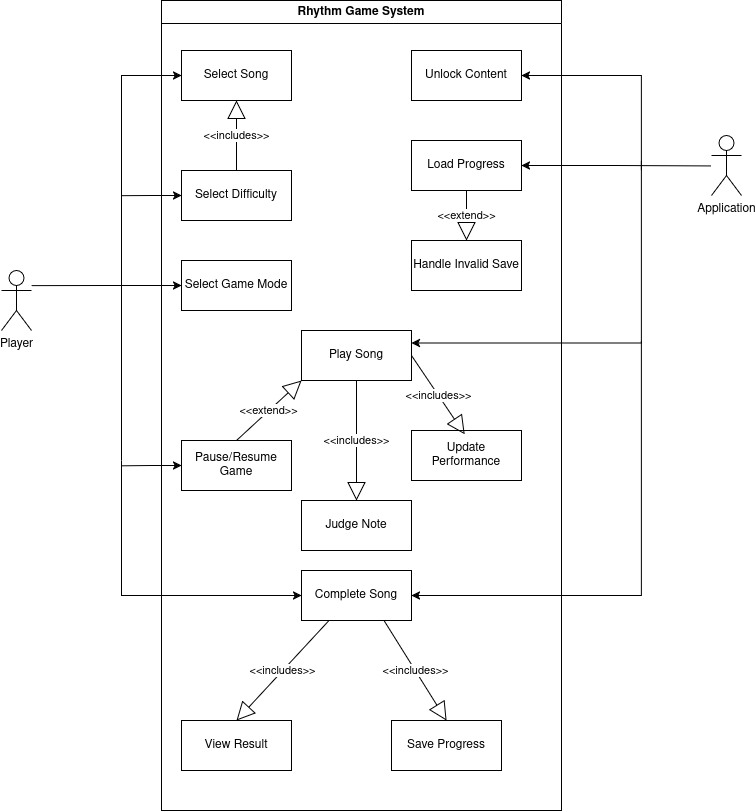
\includegraphics[width=\textwidth]{UseCase.png}
                \caption{Use Case Diagram}
            \end{figure}
            

\pagebreak

        \subsection{Written Use Case - UC4}
            \subsubsection{Primary Actor}
                Player
            
            \subsubsection{Goal}
                Play a selected song and receive timing judgements and performance feedback based on their inputs.
            
            \subsubsection{Preconditions}
                \begin{enumerate}
                    \item The application is running.
                    \item The player has selected a valid song.
                    \item The player has selected an available difficulty.
                    \item The selected chart can be loaded successfully.
                    \item A valid game mode has been selected.
                    \item A `GameSession' can be created in the initial state.
                \end{enumerate}
            

            \subsubsection{Main Success Scenario}
                \begin{enumerate}
                    \item The player selects Play from the song selection screen.
                    \item The system loads the selected chart.
                    \item The system creates a new game session using selected song, difficulty, and game mode.
                    \item The game session trasitions from `Loading' to `Playing'.
                    \item The system begins presenting notes according to their scheduled times.
                    \item The player provides an input corresponding to an upcoming note.
                    \item The system obtains the input timestamp.
                    \item The system identifies the relevant note.
                    \item The system calculates the difference between the plyer's input time and the note's scheduled time.
                    \item The system determines a timing judgement, such as `Perfect', `Great', `Good', or `Miss'.
                    \item The system applies the apporpriate behaviour for the note type. For example, a tap note is resolved by a single input, while a hold note requires the player to maintain the input for its required duration.
                    \item The system updates the player's score, combo, and accuracy.
                    \item THe updated performatnce information is displayed to the player.
                    \item Steps 6-13 repeat as the remaining notes are played.
                    \item When the chart is complete, the system transitions the game session to `Finished'.
                    \item The system creates a song result containing the player's score, accuracy, combo, and judgement information.
                    \item The result is displayed to the player.
                    \item The player's progression and result are saved.
                \end{enumerate}
            

            \subsubsection{Alternative Flows}
                \begin{itemize}
                    \item A1: Player pauses the game.
                    \begin{enumerate}
                        \item While the session is `Playing', the player selectes pause.
                        \item The system transitions the session to `Paused'.
                        \item Note progression and gameplay input processing stop.
                        \item The player selects resume.
                        \item The system transitions the session back to `Playing'.
                        \item Gameplay continues from the paused state.
                    \end{enumerate}
                    \item A2: Player completes a hold note.
                    \begin{enumerate}
                        \item The player begins the hold input withint the valid timing window.
                        \item The system records the start of the hold.
                        \item The player maintains the input for the required duration.
                        \item The system validates the hold duration.
                        \item The hold note is successfully resolve and the appropriate score is awareded.
                    \end{enumerate}
                    \item A3: Player makes a late or early input.
                    \begin{enumerate}
                        \item The player's input occurs outside the `Perfect' timing window.
                        \item The system calculates the timing difference.
                        \item The appropriate lower judgement is assigned.
                        \item The score, combo, and accuracy are updated according to the judgement.
                    \end{enumerate}
                \end{itemize}
            
            \subsubsection{Exception Flows}
                \begin{itemize}
                    \item E1: Invalid player input
                    \begin{enumerate}
                        \item The player provides an input that does not correspond to a valid control or lane.
                        \item The system rejects the input.
                        \item The system displays an appropriate feedback message where applicable.
                        \item The current game state, score, and valid notes remain unchanged.
                    \end{enumerate}
                    \item E2: Illegal game state transition
                    \begin{enumerate}
                        \item An attempt is made to perform an operation that is invalid for the current state, such as resuming a session that is already `Playing'.
                        \item The system rejectes the transition.
                        \item The session remains in its current valid state.
                        \item The system reports the error appropriately.
                    \end{enumerate}
                    \item E3: Chart cannot be loaded
                    \begin{enumerate}
                        \item The selected chart cannot be loaded or is invalid.
                        \item The system does not start the game session.
                        \item The player is informed that the song cnnat currently be played.
                        \item The player remains on the song selection screen.
                    \end{enumerate}
                \end{itemize}
            
            \subsubsection{Postconditions}
                \begin{itemize}
                    \item Successful Completion
                    \begin{enumerate}
                        \item The game session is in the `Finished' state.
                        \item Every required note has been resolved.
                        \item A song result containing the player's performance has been created.
                        \item Score, combo, accuracy, and judgement information have been calculated.
                        \item The result is displayed to the player.
                        \item The player's progression is updated.
                        \item The updated progression is saved.
                    \end{enumerate}
                    \item Unsuccessful Completion
                    \begin{enumerate}
                        \item The game session remains in a valid state or is not created.
                        \item No invalid score or progression data is stored.
                        \item The player receives appropriate feedback about the failure.
                    \end{enumerate}
                \end{itemize}

\pagebreak

\section{Initial Class Diagram}
    \begin{figure}[H]
        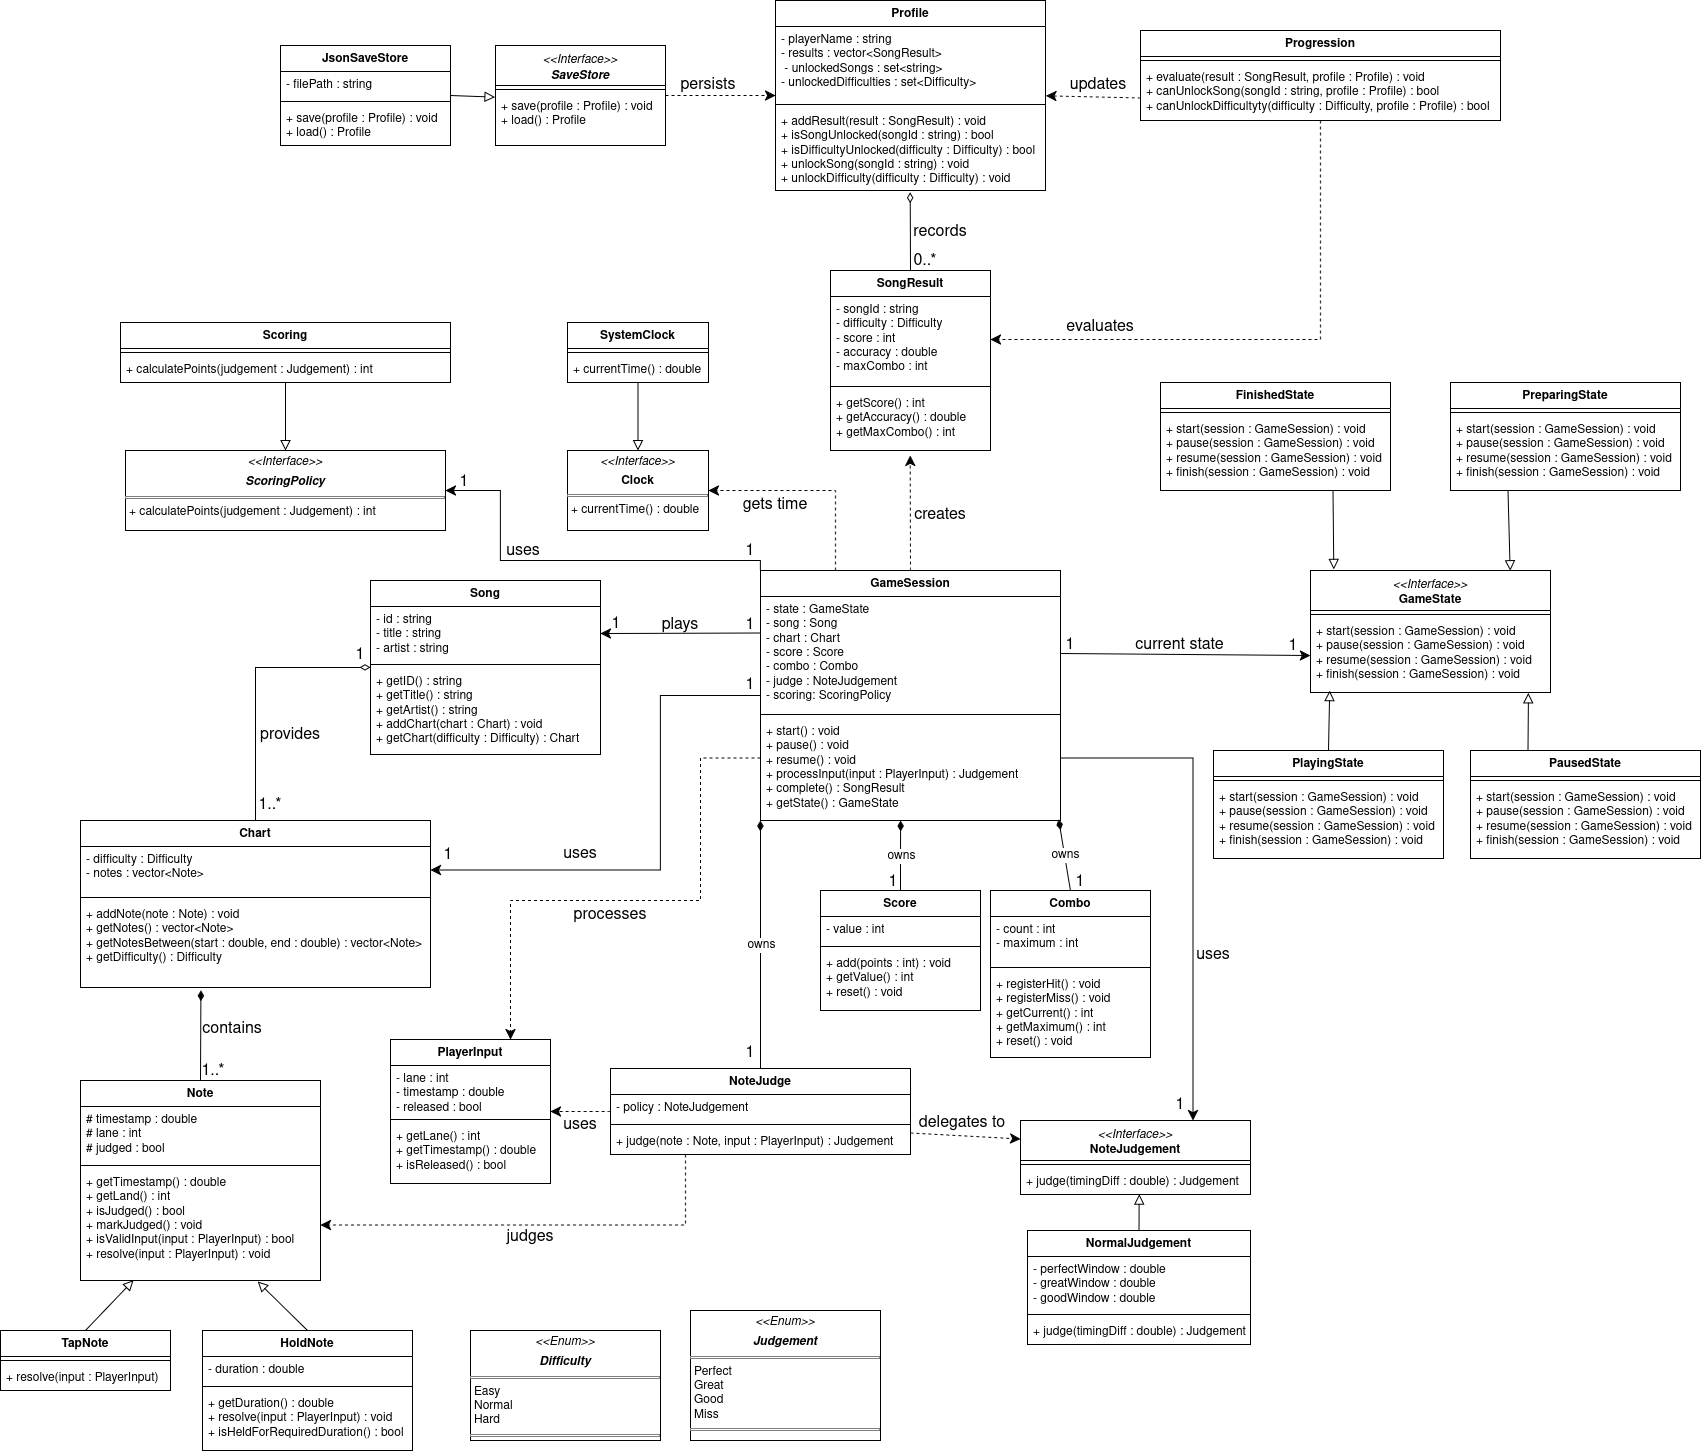
\includegraphics[width=\textwidth]{ClassDiagram.png}
        \centering
        \caption{Initial Class Diagram}
    \end{figure}
    Since the diagram is big, you may not clearly see everything on this document. \\
    If that's the case, see \href{https://github.com/jspace418/CS3307_Project/blob/main/D1/img/ClassDiagram.png}{image on github} for details.

\pagebreak

\section{Sequence Diagram}
    \begin{figure}[H]
        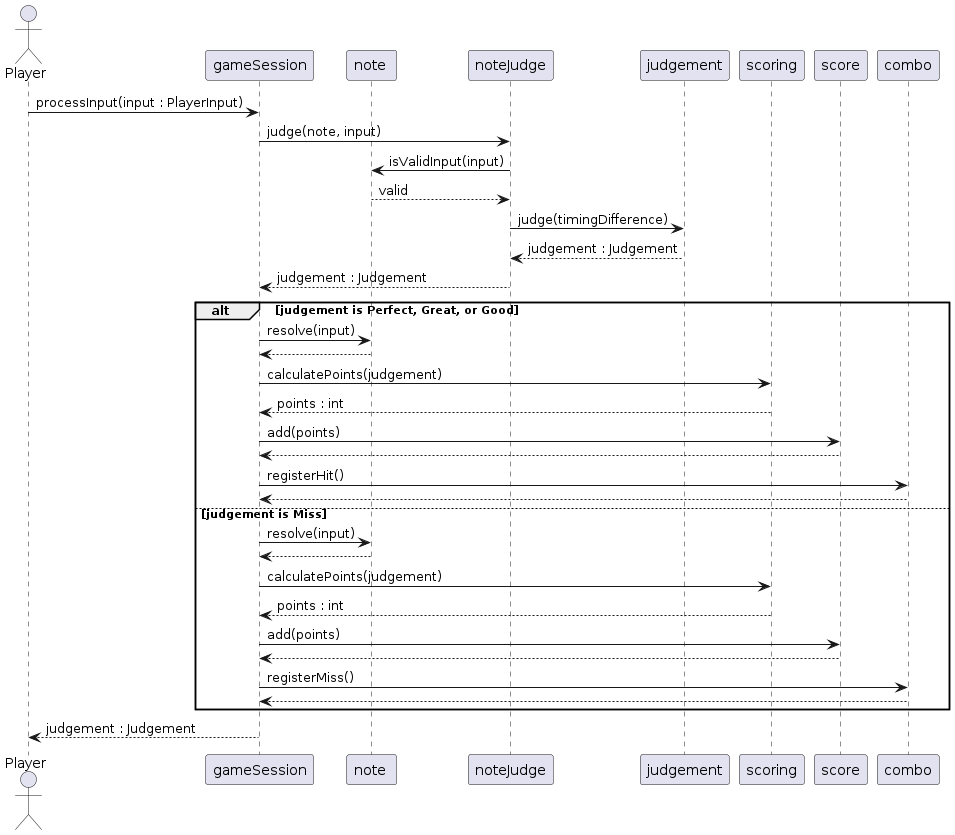
\includegraphics[width=\textwidth]{SequenceDiagram.png}
        \centering
        \caption{Sequence Diagram}
    \end{figure}
    If you can't read some texts, see \href{https://github.com/jspace418/CS3307_Project/blob/main/D1/img/SequenceDiagram.png}{image on github}.

\pagebreak

\section{Architecture Overview}
    \tab The system will use a modular, layered architecture consisting of three core domain modules: Song and Chart, Gameplay, and Progression.
    The system will also contain Qt-based presentation layer in \texttt{ui/} and an external service boundary within \texttt{core/} for persistence and time-related dependencies.\\
    \tab The Song and Chart module is responsible for representing the available songs, difficulty-based charts, and individual notes. A Song contains one or more Chart objects, while Chart contains Note objects.
    Note is an abstract class with TapNote and HoldNote implementations. This module contains the data and behaviour required to describe what the player must perform, but does not handle user interface concerns or the overall game session. \\
    \tab The Gameplay module controls an active game session. GameSession coordinates the current song, chart, score, combo, note judgement, scoring policy, and game state transitions.
    NoteJudge determines the result of player input using NoteJudgement abstraction, while ScoringPolicy determines the points awareded for a judgement.
    The GameState and its states enforce valid game session transitions. The Gameplay module depends on the Song and Chart module because it processes the notes contained in a selected chart. \\
    \tab The Progression module manages information that persists between gameplay sessions.
    Profile stores the player's results and unlocked content, SongResult represents the outcome of a completed song, and Progression evaluates results to determine whether songs or difficulties should be unlocked.
    The Progression module therefore receives results from Gameplay and maintains the player's progression. \\
    \tab The UI layer is located in \texttt{ui/} and forms a strict boundary around the core domain.
    It will contain the Qt 6 views and controllers used to display menus, song selection, gameplay, and results.
    UI classes may depend on classes and interfaces in \texttt{core/}, but the reverse dependency is prohibited.
    For example, the UI may translate a keyboard event into a PlayerInput and pass it to GameSession, but GameSession will not depend on Qt classes.
    This keeps the domain independently compilable and testable. \\
    \tab The external boundary is handled through two interfaces in \texttt{core/}: SaveStore and Clock.
    SaveStore abstracts persistence so that the domain does not depend directly on a particular file format.
    Its real implementation will be JsonSaveStore, which saves and loads the player's Profile from a file.
    Similarly, Clock abstracts access to the current time. SystemClock will provide the real implementation during gameplay.
    Consequently, the core domain depends on these abstractions rather than directly on external services.

\pagebreak

\section{Design Approach \& Candidate Patterns}
    \tab Encapsulation will be used to keep domain state private and expose only operations that maintain valid state.
    For example, Score will control changes to its score value through operations such as \texttt{add()}, while GameSession will control valid transitions between its game states rather than allowing other classes to directly modify its state. \\
    \tab Inheritance will be used where there is genuine is-a relationship and shared behaviour.
    TapNote and HoldNote will inherit from the abstract Note class because both represent playable notes but have different resolution behaviour. \\
    \tab Polymorphism will allow GameSession and other domain classes to work with abstractions rather than concrete implementations.
    For example, NoteJudge uses the NoteJudgement interface, allowing a NormalJudgement implementation to be replaced by another judgement policy without modifying NoteJudge.
    GameSession similarly uses the ScoringPolicy interface rather than depending directly on Scoring.
    This supports adding alternative gameplay rules without modifying existing classes. \\
    \tab Abstraction will be important at variation points and external boundaries.
    NoteJudgement, ScoringPolicy, GameState, Clock, and SaveStore expose only the operations that clients need while hiding their implementation details.
    The Clock and SaveStore abstractions also ensure that the core domain does not depend directly on the system. \\
    \tab Where possible, the design will favour composition over inheritance.
    For example, GameSession contains Score, Combo, and NoteJudge rather than inheriting from these classes.
    Composition allows each responsibility to change independently and avoids creating a deep inheritance hierarchy.
    Inheritance is only reserved for cases such as TapNote/HoldNote mentioned above. \\
    \tab The design will be primarily influenced by the SOLID principles:
    \begin{itemize}
        \item \textbf{Single Responsibility:} classes such as NoteJudge, Score, Combo, Progression, and GameSession will have distinct responsibilities rather than combining unrelated gameplay logic.
        \item \textbf{Open/Closed:} judgement and scoring behaviour can be extended by addding implementations of NoteJudgement and ScoringPolicy without modifying their clients.
        \item \textbf{Liskov Substitution:} concrete notes, judgement policies, and game states should be usable wherever their corresponding abstractions are expected.
        \item \textbf{Interface Segregation:} interfaces such as Clock and SaveStore will expose only the operations needed by their clients.
        \item \textbf{Dependency Inversion:} GameSession and other domain classes will depend on abstractions such as Clock, SaveStore, NoteJudgement, and ScoringPolicy rather than concrete implementations.
    \end{itemize} 
    \tab The state pattern is the strongest current pattern design candidate because the game session has a clearly defined lifecycle with guarded transitions.
    Abstract factory and factory method address separate object-creation problems: constructing compatible gameplay policies and constructing different note types.
    These choices will be revisited during Deliverable 2 as the implementation and class responsibilities become clearer.


\section{Milestone Plans \& Risks}
    \tab D2 will provide about half of the final system, with priority given to establishing the complete core architecture and a working gameplay loop.
    The remaining features will then build on this foundation rather than requiring major architectural changes late in the project.
    \begin{table}[H]
        \centering
        \begin{tabular}{@{}lll@{}}
            \toprule
            Requirements & D2 Target & Planned implementation \\ 
            \midrule
            FR1  & Yes     & Song selection screen with available songs \\
            FR2  & Yes     & Difficulty selection for selected song \\
            FR3  & Partial & Chart loading logic and draw notes on screen \\
            FR4  & Partial & NoteJudge timing window \\
            FR5  & Yes     & TapNote and HoldNote implementation \\
            FR6  & Partial & Score and combo calculation \\
            FR7  & Partial & Core GameState lifecycle, \\
                 &         & and UI integration for main transitions \\
            FR8  & Partial & SaveStore abstraction, JsonSaveStore logic, and \\ 
                 &         & basic profile/result persistence \\
            FR9  & No      & Optional feature deferred until all FR is complete \\
            FR10 & No      & Planned for D3 \\
            FR11 & Partial & Persistence error detection and failure behaviour \\
            \bottomrule
        \end{tabular}
        \caption{Milestone Planning Table}
    \end{table}
    \tab The first risk is that gameplay architecture getting too complex. 
    This could potentially require major modification to notes, scoring, judgement, or game states and make D2/D3 implementation difficult to maintain.
    Possible mitigation is to implement a small end-to-end gameplay slice early. Keep GameSession as a coordinator and separate judgement, scoring, notes, state management, andn persistence
    behind focused classes and iterfaces. \\
    \tab The second risk is that timing and input handling being difficult to implement reliably.
    In rhythim games, timing is the key. And inaccurate timing could make the core system mechanic unreliable and difficult to test.
    Possible mitigation is to separate timing behind the Clock interface and represent input using PlayerInput class. By creating second Clock interface, we can use that to create deterministic tests for timing windows
    and note judgements rather than relying on real-time gameplay during testing. \\
    \tab The last risk is required features and teseting taking longer than expected. Some requirements taking longer to implement could consume time to the point where it puts D3 deadlines at risk.
    Possible mitigation is to prioritizing rubric requirements over features. Optional features such as FR9 will be dropped first if needed, followed by
    non-essential gameplay polish.



\section{Design Depth Profile}


\end{document}